\subsection{SPI-Master}
\label{sec:SPIMaster}

The microcontroller have to share information with the FPGA, and according to the requirements mentioned in section \ref{sec:Primaryrequirements}, this communication has to happen using Serial Peripheral Interface (SPI). The protocol will operate as descriped in section \ref{sec:SPIcommunication}. It is therefore important that this link never will be a bottleneck for the system application. 

The requirements of the minimum bit-rate depends om what data that needs to be send, and how often it needs to send it. Since the PID-controller is placed in the FPGA, the application only needs to update the current position once every 5 ms, which is the minimal delay that freeRTOS can put on a task. 

The length of the messages send is defined by the driver placed in the FPGA. As described in section \ref{sec:Implementation} all messages will have the length of 14 bits. Updating both pan and tilt requires two messages giving  considering the all other 

set the limit for the respoce time from the user to the system

, What are the bit rate requirements. 
25 ms sekundær
500 ms primær
using the internal freescale spi module or making it from scratch
- the avantage of full control

designing the statemashine

Mesure the performance 



A state is only a state if you have to wait till you move on


% full dreasd task diagram
\begin{figure}
	\centering
	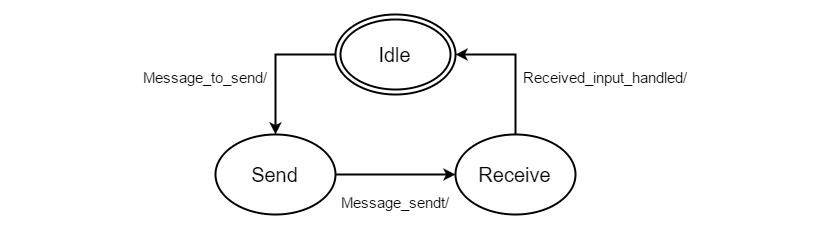
\includegraphics[scale = 0.7] {Billeder/SPI-master}
	\caption{The SPI-master state machine}
	\label{fig:SPI-master}
\end{figure}



